% \section{Research}
% \begin{frame}{Setup}
% 	\begin{itemize}
% 		\item EMNIST (Knowns: Digits, Unknowns: Letters)
% 		\item Cross product of parameters
% 		\item Agglomerative Clustering
% 		\item Fixed numbers of clusters
% 	\end{itemize}
% \end{frame}
%
\begin{frame}{Research Questions 2}
	\texttt{RQ2}: Can clustering improve OpenMax's performance?
\end{frame}

\begin{frame}{Results RQ2 ($\gamma$)}
	\centering
	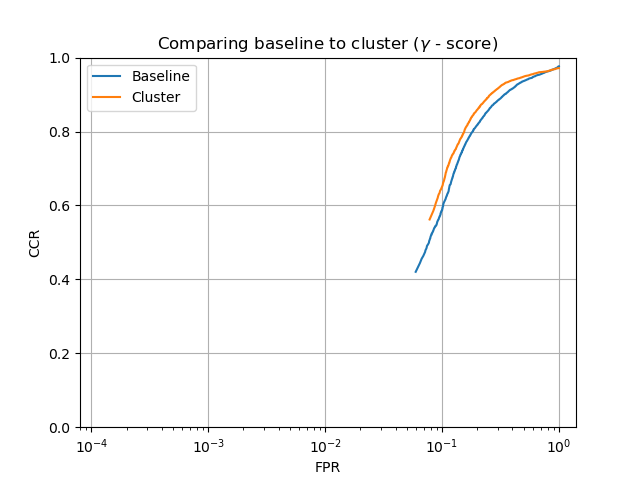
\includegraphics[width=0.65\textwidth]{figures/compare_gamma.png}
	\footnotesize{
		\begin{tabularx}{\textwidth}{ |X|X|X|X|X|X|X|X| }
			\hline
			Rank & $\alpha$ & $\eta$ & $\kappa$ & $k_{\text{Input}}$ & $k_{\text{Feat}}$ & $\gamma$ & $\Sigma$ \\
			\hline
			1    & 7        & 100    & 0.7      & 1                  & 5                 & 0.829    & 4.391    \\
			2    & 7        & 1000   & 1.0      & 1                  & 1                 & 0.805    & 4.272    \\

			\hline
		\end{tabularx}
	}
\end{frame}

\begin{frame}{Results RQ2 ($\Sigma$)}
	\centering
	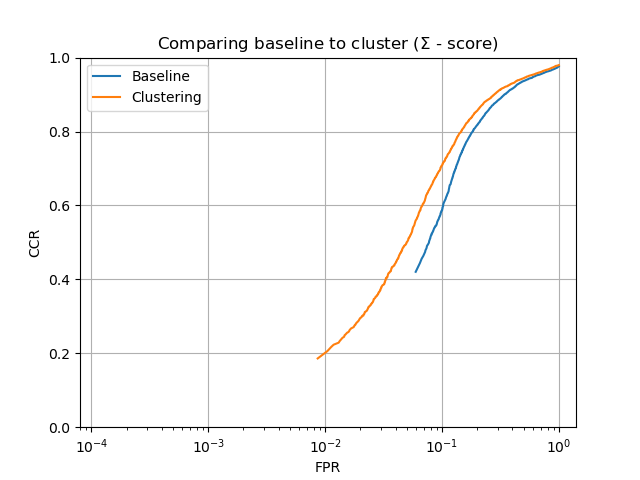
\includegraphics[width=0.65\textwidth]{figures/compare_sigma.png}
	\footnotesize{
		\begin{tabularx}{\textwidth}{ |X|X|X|X|X|X|X|X| }
			\hline
			Rank & $\alpha$ & $\eta$ & $\kappa$ & $k_{\text{Input}}$ & $k_{\text{Feat}}$ & $\gamma$ & $\Sigma$ \\
			\hline
			1    & 7        & 750    & 1.25     & 1                  & 6                 & 0.768    & 4.450    \\
			2    & 7        & 1000   & 1.0      & 1                  & 1                 & 0.805    & 4.272    \\
			\hline
		\end{tabularx}
	}
\end{frame}

\begin{frame}{Research Questions 3}
	\texttt{RQ3}: If clustering improves OpenMax, which clustering type is optimal, and by using which parameters?
\end{frame}

\begin{frame}{Results RQ3 ($\gamma$)}
	\centering
	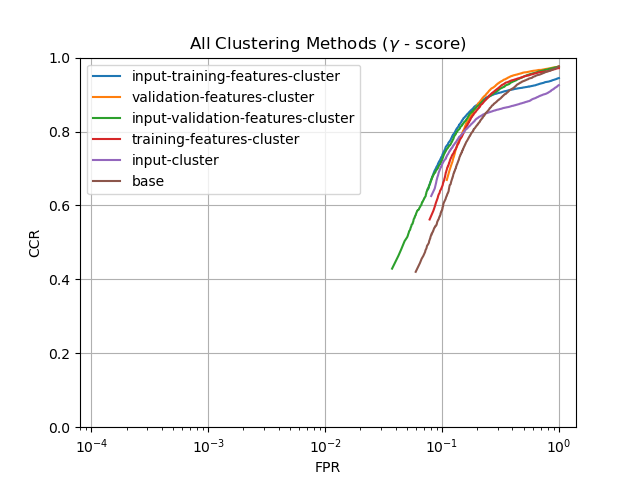
\includegraphics[width=0.5\textwidth]{figures/all_methods_gamma.png}
	\footnotesize{
		\begin{tabularx}{\textwidth}{ |X|X|X|X|X|X|X|X|X| }
			\hline
			Rank & Type & $\alpha$ & $\eta$ & $\kappa$ & $k_{\text{Input}}$ & $k_{\text{Feat}}$ & $\gamma$ & $\Sigma$ \\
			\hline
			1    & ITFC & 5        & 100    & 0.7      & 2                  & 3                 & 0.841    & 3.666    \\
			2    & VFC  & 7        & 10     & 0.5      & 1                  & 5                 & 0.834    & 3.774    \\
			3    & IVFC & 5        & 100    & 1.25     & 2                  & 6                 & 0.834    & 4.478    \\
			4    & TFC  & 7        & 100    & 0.7      & 1                  & 5                 & 0.829    & 4.391    \\
			5    & IC   & 5        & 100    & 0.5      & 2                  & 1                 & 0.822    & 4.247    \\
			6    & base & 7        & 1000   & 1.0      & 1                  & 1                 & 0.805    & 4.272    \\
			\hline
		\end{tabularx}
	}

\end{frame}

\begin{frame}{Results RQ3 ($\Sigma$)}
	\centering
	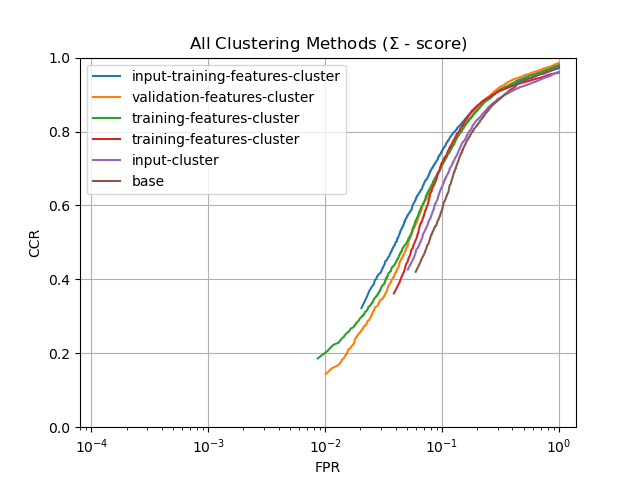
\includegraphics[width=0.5\textwidth]{figures/all_methods_sigma.png}
	\footnotesize{
		\begin{tabularx}{\textwidth}{ |X|X|X|X|X|X|X|X|X|}
			\hline
			Rank & Type & $\alpha$ & $\eta$ & $\kappa$ & $k_{\text{Input}}$ & $k_{\text{Feat}}$ & $\gamma$ & $\Sigma$ \\
			\hline
			1    & IVFC & 5        & 100    & 1.0      & 2                  & 6                 & 0.828    & 4.483    \\
			2    & VFC  & 7        & 250    & 1.25     & 1                  & 5                 & 0.742    & 4.475    \\
			3    & TFC  & 7        & 750    & 1.25     & 1                  & 6                 & 0.768    & 4.450    \\
			4    & ITFC & 5        & 1000   & 1.5      & 2                  & 3                 & 0.827    & 4.423    \\
			5    & IC   & 7        & 500    & 1.0      & 2                  & 1                 & 0.812    & 4.307    \\
			6    & base & 7        & 1000   & 1.0      & 1                  & 1                 & 0.805    & 4.272    \\
			\hline
		\end{tabularx}
	}
\end{frame}
